\subsection{Across Policies and Execution Environments}
\label{sec:main_results}
\begin{table}[!t]
\centering
\small
\setlength{\tabcolsep}{6pt}
\caption{Task success rate (\%) in simulation. All methods run the same base policy under the benchmark's standard physical step limit, including recovery motion: 300 steps on SimplerEnv Bridge and each task's registered limit on RoboCasa. Overall pools all trials of a benchmark. Best result per row in bold. $\dagger$Adapted baselines; see \cref{sec:exp_setup}.}
\label{tab:main-results}
\begin{tabular}{@{}llrcccc@{}}
\toprule
 & & & \multicolumn{3}{c}{Baselines} & \\
\cmidrule(lr){4-6}
Policy & Task & $N$ & Base & RoboMonkey$^\dagger$ & CycleVLA$^\dagger$ & ACRO \\
\midrule
GR00T N1.7 & Carrot on Plate    & 60 & 50.0 & 31.7 & 48.3 & \textbf{68.3} \\
{\footnotesize SimplerEnv Bridge} & Eggplant in Basket & 60 & 36.7 & 50.0 & \textbf{66.7} & 51.7 \\
           & Spoon on Towel     & 60 & \textbf{93.3} & 90.0 & \textbf{93.3} & \textbf{93.3} \\
           & Stack Cube         & 60 & 18.3 & 18.3 & 13.3 & \textbf{26.7} \\
\cmidrule(l){2-7}
           & Overall            & 240 & 49.6 & 47.5 & 55.4 & \textbf{60.0} \\
\midrule
$\pi_{0.5}$ & Open/Close/Slide        & 250 & 64.4 & 66.8 & 65.6 & \textbf{76.0} \\
{\footnotesize RoboCasa} & Pick-and-Place & 250 & 64.0 & \textbf{68.0} & 56.0 & 65.2 \\
            & Control Operation       & 100 & 43.0 & 52.0 & 40.0 & \textbf{55.0} \\
\cmidrule(l){2-7}
            & Overall                 & 600 & 60.7 & 64.8 & 57.3 & \textbf{68.0} \\
\bottomrule
\end{tabular}
\end{table}


\paragraph{On Simulation Benchmarks.}
We evaluate ACRO across two pretrained VLAs and two simulation environments to test its use across different policies and manipulation settings. Table~\ref{tab:main-results} covers tabletop manipulation with GR00T~N1.7 on SimplerEnv Bridge and household interactions with $\pi_{0.5}$ on RoboCasa. ACRO raises overall success from 49.6\% to 60.0\% on SimplerEnv and from 60.7\% to 68.0\% on RoboCasa. It also exceeds RoboMonkey and CycleVLA overall in both settings. RoboMonkey ranks eight policy samples per query with the same Critic, while CycleVLA uses external VLM inference for recovery. With each base policy fixed and all return motion charged to the physical budget, these gains show that ACRO applies across distinct VLA backbones, environments, and task types.

\Needspace{14\baselineskip}
\begin{wraptable}{r}{0.47\linewidth}
\centering
\normalsize
\setlength{\tabcolsep}{5pt}
\caption{Real-robot success rate (\%).}
\label{tab:real-robot}
\vspace{2pt}
\begin{tabular}{@{}lrcc@{}}
\toprule
Task & $N$ & Base & ACRO \\
\midrule
Pick and Place & 20 & 70.0 & 80.0 \\
Stack Cube     & 20 & 20.0 & 55.0 \\
Press Button   & 20 & 40.0 & 60 \\
\midrule
Overall        & 60 & 43.3 & 65 \\
\bottomrule
\end{tabular}
\end{wraptable}

\paragraph{Real-Robot Evaluation.}
Physical retraction must bring the robot back to a useful configuration despite sensing noise and actuation error. We test this requirement on a real robot using $\pi_{0.5}$ for pick and place, cube stacking, and button pressing (Table~\ref{tab:real-robot}). ACRO improves success on all three tasks, with the largest gain on cube stacking (20.0\% to 55.0\%). Across 60 trials, it completes 39 tasks compared with 26 for Base VLA, raising success from 43.3\% to 65.0\%. The improvement under real-world execution conditions shows that physical return and renewed policy execution can be used together for successful recovery.
\finishwrap

\Needspace{20\baselineskip}
\begin{wrapfigure}{r}{0.48\linewidth}
\vspace{-4pt}
\captionsetup{justification=raggedright,singlelinecheck=false}
\centering
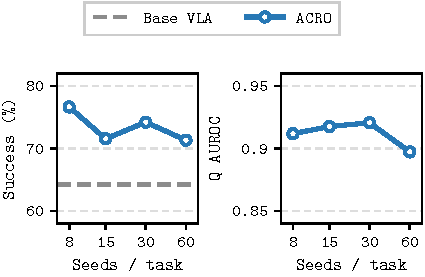
\includegraphics[width=\linewidth]{figures/data_scale.pdf}
\caption{\textbf{A small rollout set suffices to train the Critic.} Success and AUROC of minimum rollout Q over three tasks at $2H_{\mathrm{ref}}$.}
\label{fig:data-scale}
\end{wrapfigure}

\paragraph{Critic Training Cost.}
\label{sec:critic-data}
The Critic is trained from rollouts of the deployed policy. To measure the data needed to build it, we vary the training set from 8 to 60 seeds per task across 12 tasks, training one Critic with joint Q and V heads per size and fixing the validation and calibration sets at 180 and 300 rollouts. We evaluate on three RoboCasa tasks with 150 trials per task at $2H_{\mathrm{ref}}$ (\cref{app:protocol}). Figure~\ref{fig:data-scale} shows that ACRO exceeds Base VLA at every tested size. With 8 seeds per task, it reaches 76.7\% success using 96 training rollouts; AUROC ranges from 0.897 to 0.921 across sizes. These results show that a small training set is sufficient to build a Critic that improves task completion.
\finishwrap[3]

\Needspace{23\baselineskip}
\subsection{Critic-Guided Recovery}
\label{sec:analysis}
The preceding results show that ACRO improves completion across the evaluated policies and environments. We now examine the role of its recovery strategy, the successes gained through intervention, and the execution that follows a return.

\Needspace{16\baselineskip}
\begin{wraptable}{r}{0.49\linewidth}
\vspace{-4pt}
\captionsetup{justification=raggedright,singlelinecheck=false}
\centering
\small
\setlength{\tabcolsep}{4pt}
\caption{\textbf{ACRO improves on scheduled rewinds.} All 600 RoboCasa trials at $H$; returns and return steps are trial means.}
\label{tab:periodic-rewind}
\begin{tabular}{@{}lrrr@{}}
\toprule
Method & Success (\%) & Returns & Steps \\
\midrule
Base VLA & 60.7 & 0 & 0 \\
Periodic & 59.5 & 1.04 & 92.7 \\
\rowcolor{linkblue!12}
ACRO & 68.0 & 1.06 & 46.3 \\
\bottomrule
\end{tabular}
\end{wraptable}

\paragraph{Scheduled Rewinds.}
A fixed rewind schedule also gives the policy repeated attempts. We compare this strategy with ACRO to examine the benefit of using Critic estimates to guide recovery. Periodic rewind uses fixed intervals, fixed look-back distances, and reverse replay, while ACRO uses Q to activate recovery and V to select a target reached through Trajectory Retraction. On the same 600 RoboCasa trials at the standard physical budget $H$, Periodic completes 59.5\% of trials, compared with 60.7\% for Base VLA and 68.0\% for ACRO (Table~\ref{tab:periodic-rewind}). Periodic and ACRO initiate similar numbers of returns per trial (1.04 and 1.06), while ACRO uses about half as many return steps (46.3 versus 92.7). The Critic-guided strategy thus turns a similar number of recovery attempts into more completed tasks with less return motion.
\finishwrap

\Needspace{15\baselineskip}
\begin{wraptable}{r}{0.53\linewidth}
\vspace{-4pt}
\captionsetup{justification=raggedright,singlelinecheck=false}
\centering
\small
\setlength{\tabcolsep}{4.5pt}
\caption{\textbf{Gained successes exceed losses.} RoboCasa trials at $H$, relative to Base. Policy-step means use the 46 shared successes after ACRO's first alarm.}
\label{tab:recovery-summary}
\begin{tabular}{@{}lrrrr@{}}
\toprule
 & \multicolumn{2}{c}{Outcome changes} & \multicolumn{2}{c}{Mean rollout steps} \\
\cmidrule(lr){2-3}\cmidrule(l){4-5}
Category & Gained & Lost & Base & ACRO \\
\midrule
Open/close & 33 & 4 & 362.6 & 296.1 \\
Pick/place & 17 & 14 & 387.0 & 345.5 \\
Control & 20 & 8 & 139.3 & 157.7 \\
\midrule
\textbf{Overall} & \textbf{70} & \textbf{26} & \textbf{327.9} & \textbf{287.3} \\
\bottomrule
\end{tabular}
\end{wraptable}

\paragraph{Gained and Lost Successes.}
An intervention can recover a failed execution, but it can also interrupt one that would succeed. To examine this balance, Table~\ref{tab:recovery-summary} decomposes the outcome differences over the RoboCasa trials at $H$. ACRO succeeds on 70 trials where Base fails and fails on 26 where Base succeeds, giving 44 additional completions. Periodic rewind gains 50 successes and loses 57. ACRO's net gain is positive in every category: +29 on open/close, +12 on control, and +3 on pick and place. Thus, the overall improvement reflects more gained than lost successes across the three categories. The comparison protocol is detailed in Appendix~\ref{app:recovery-timing}.
\finishwrap

\Needspace{8\baselineskip}
\begin{figure}[!t]
\centering
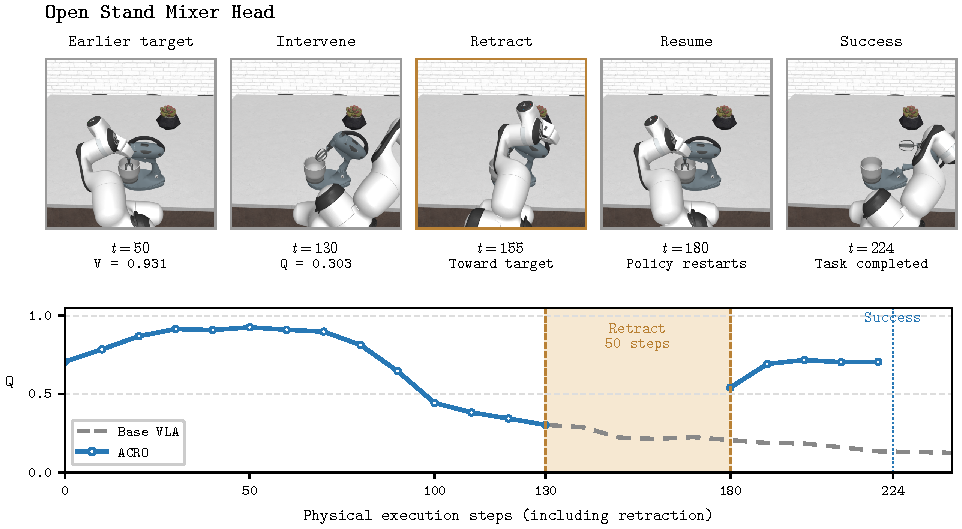
\includegraphics[width=\linewidth]{figures/qualitative_recovery.pdf}
\caption{\textbf{Retraction enables a successful re-approach.} ACRO intervenes at step 130, spends 50 steps returning toward the target at step 50, and succeeds at step 224; paired Base VLA times out at 1,000. Q curves show the first 240 steps, with no queries during retraction. Frames show the recorded execution replayed in the simulator.}
\label{fig:qualitative-recovery}
\end{figure}

\paragraph{Recovery through a New Approach.}
Figure~\ref{fig:qualitative-recovery} shows how a return can lead to a successful continuation on Open Stand Mixer Head. ACRO intervenes at step 130 as estimated continuation success declines, then spends 50 steps returning toward an earlier target. The policy resumes and opens the mixer head after another 44 steps. Base VLA continues with low Q estimates and fails within 1,000 steps. In this example, returning to a previously visited state allows the frozen policy to make a new approach and complete the task.

\paragraph{Execution Efficiency after Returning.}
Returning moves the robot to an earlier point along its path. If the policy then needs fewer execution steps to finish, that return has provided a more productive starting point for the next attempt. We examine the 46 trials in which both Base and ACRO succeed after ACRO's first-alarm step. From that step onward, Base uses 327.9 policy steps on average and ACRO uses 287.3, counting every retry (Table~\ref{tab:recovery-summary}). The reduction comes from open/close and pick-and-place tasks; control tasks use more policy steps under ACRO. Including return motion gives ACRO 339.9 physical steps. The lower policy-step count shows how execution after returning can reach success with fewer policy execution steps, while the physical total accounts for the movement needed to reach the re-entry state.

\Needspace{24\baselineskip}
\subsection{Test-Time Scaling and Retraction Cost}
\label{sec:data-retraction}
ACRO uses additional execution time for renewed attempts. We examine how task completion scales with this budget and how Trajectory Retraction reduces the steps spent returning between attempts.

\begin{wrapfigure}{r}{0.46\linewidth}
\vspace{-12pt}
\captionsetup{justification=raggedright,singlelinecheck=false}
\centering
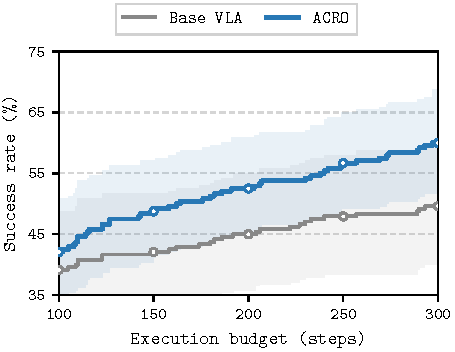
\includegraphics[width=0.94\linewidth]{figures/budget_curves.pdf}
\caption{\textbf{Success grows with budget.} Bands: 95\% bootstrap intervals.}
\label{fig:budget-curves}
\end{wrapfigure}

\paragraph{Test-Time Scaling.}
Additional execution time gives ACRO more opportunities to return and try again. We examine test-time scaling by increasing the physical execution budget and measuring how many additional tasks are completed. Figure~\ref{fig:budget-curves} scores the same 240 SimplerEnv executions at successive step limits up to 300, including all retraction steps. Within the first 100 steps, ACRO and Base VLA complete 101 and 94 trials. Over the remaining 200 steps, ACRO adds 43 completions and Base adds 25. On Eggplant in Basket, Base adds no success after step 100 while ACRO adds five; task-level curves appear in \cref{fig:budget-curves-tasks}. Thus, ACRO converts additional execution budget into further successes through renewed attempts.
\finishwrap[3]

\Needspace{14\baselineskip}
\begin{wraptable}{r}{0.49\linewidth}
\vspace{-4pt}
\captionsetup{justification=raggedright,singlelinecheck=false}
\centering
\small
\setlength{\tabcolsep}{3pt}
\caption{\textbf{Shortcuts reduce return cost.} Paths at $2H_{\mathrm{ref}}$: success (\%), mean return steps, and target reach (\%).}
\label{tab:rewind-path}
\begin{tabular}{@{}lrrr@{}}
\toprule
Path & Success & Steps & Reach \\
\midrule
Reverse replay & 70.7 & 62.0 & 86.2 \\
RDP-simplified & 70.9 & 43.4 & 80.5 \\
Straight line & 70.7 & 20.6 & 64.1 \\
\rowcolor{linkblue!12}
Ours & 71.3 & 32.4 & 85.4 \\
\bottomrule
\end{tabular}
\end{wraptable}

\paragraph{Retraction Path.}
Replaying the recorded path spends steps on detours made during the original attempt. We compare reverse replay with an RDP-simplified path, a shortcut within a tube around visited positions, and a straight line to the target. All variants use three RoboCasa tasks with 150 trials per task at $2H_{\mathrm{ref}}$ (\cref{app:protocol}). Table~\ref{tab:rewind-path} shows that the visited-tube shortcut reduces the mean return from 62.0 to 32.4 steps while retaining similar target reach (86.2\% versus 85.4\%). A straight line is shorter (20.6 steps), but reaches the target in only 64.1\% of returns. Task success stays between 70.7\% and 71.3\% across paths. The visited-tube shortcut therefore saves return steps while preserving reliable access to the target.
\finishwrap
